\chapter{Litigation Funding, Class Actions and Claims as Assets}
\label{ch:funding}

\section{Claims are assets}

A legal claim is a risky asset. Its owner holds a right to a payment that will be made only if the claim succeeds, after a delay, net of costs. Like any risky asset it has an expected value, a variance and a correlation with other assets, and it can be bought, sold, financed and insured. For most of the history of the common law, the doctrines of maintenance and champerty forbade strangers from funding litigation in return for a share of the proceeds, on the ground that it encouraged speculative and oppressive suits. Those doctrines have been relaxed or abolished in most of the common law world, and third party litigation funding is now an industry measured in billions. This chapter applies the decision theory of this book to the funding, aggregation and valuation of claims, which are among the most important developments in modern litigation.\index{litigation funding}

\section{Valuing a claim}

The expected value of a claim to its owner is
\begin{equation}
V = \sum_k \Prob(\text{outcome } k)\,\big(\text{recovery}_k - \text{costs}_k\big)\,e^{-r t_k},
\end{equation}
summed over the possible outcomes, including settlement at various stages, judgment for the claimant at various amounts, and judgment for the defendant. The probabilities come from the analysis of issues described in Chapters~\ref{ch:pleadings} and~\ref{ch:pleadingscases}; the recoveries from the damages analysis of Chapter~\ref{ch:damages}; the costs from the rules of Chapter~\ref{ch:systemcosts}; and the timings from the court's calendar. Each input is uncertain, and a Bayesian valuation reports a distribution, not a number.

\section{The funder's decision}

\subsection{A single claim}

A funder that pays a claimant's costs in exchange for a share of the recovery faces a bet. If the claim succeeds, the funder typically receives historically a multiple of its investment or a percentage of the damages, whichever is greater; if it fails, the funder loses its investment and, under the English costs rule, may be liable for the defendant's costs, usually covered by after the event insurance\index{after the event insurance}. With probability of success $p$, return multiple $m$ on success and loss of the stake on failure, the expected return per unit invested is $pm - 1$. A funder requiring an expected return of fifty per cent over the life of the claim on a claim with a sixty per cent chance needs $m \ge 2.5$. In the net odds $b = m - 1$ of the Kelly example below, the portfolio example ($m = 3$) and the Kelly example ($b = 2$) are the same claim.

\subsection{Portfolios}

A single claim is a highly risky asset: the funder either multiplies its money or loses it all. Funders reduce risk by holding portfolios of claims whose outcomes are not strongly correlated. Figure~\ref{fig:funding} shows the distribution of returns for a funder holding one, five and twenty independent claims, each with a sixty per cent chance of returning three times the stake. The expected return is the same; the variance falls with the number of claims. A funder with twenty independent claims almost never loses money overall. Correlation matters: claims against the same defendant, or turning on the same question of law, can fail together, and a portfolio built from them is riskier than its size suggests.\index{portfolio of claims}

\begin{figure}[t]
\centering
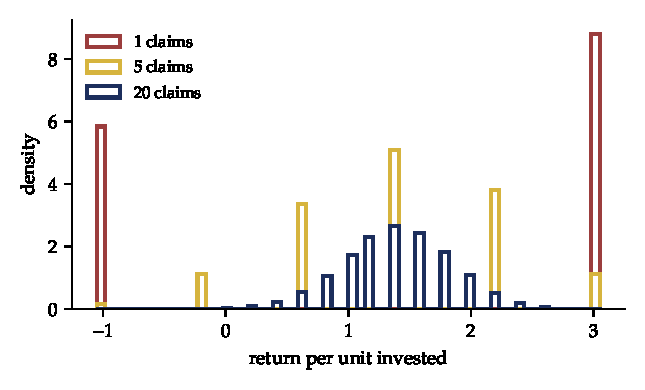
\includegraphics[width=\linewidth]{fig_funding}
\caption{Simulated return per unit invested for a funder holding one, five and twenty independent claims, each succeeding with probability $0.6$ and returning three times the stake. Diversification narrows the distribution without changing its mean.}
\label{fig:funding}
\end{figure}

\subsection{How much to invest}

How much of its capital should a funder commit to a single claim? The Kelly criterion, which maximises the expected logarithm of wealth and so the long run growth rate, gives the answer for a sequence of independent bets: invest a fraction
\begin{equation}
f^\ast = \frac{p\,b - (1-p)}{b}
\end{equation}
of capital, where $b$ is the net odds, the profit per unit staked on success. With $p = 0.6$ and $b = 2$, the Kelly fraction is $0.4$. This is the criterion of \citet{kelly1956}. In practice funders bet much less than the full Kelly fraction, because their estimates of $p$ are optimistic and overestimating $p$ leads to overbetting, which lowers long run growth and can make it negative, because their utility is more risk averse than the logarithm, and because they face limits on drawdowns. Fractional Kelly betting is the standard response \citep{maclean2011}. Posterior uncertainty about $p$ does not by itself reduce the fraction: expected log wealth is linear in $p$, so only the posterior mean of $p$ enters, and the optimal fraction is the Kelly fraction at that mean.\index{Kelly criterion}

\section{The law of funding}

\subsection{England after PACCAR}

In \emph{R (PACCAR Inc) v Competition Appeal Tribunal} the Supreme Court held in 2023 that litigation funding agreements under which the funder's return was calculated as a percentage of damages were damages based agreements within the meaning of the statute regulating them, and so were unenforceable unless they complied with the regulations, which most did not \citep{paccar2023}. The decision threatened the enforceability of a large number of existing agreements, particularly in collective proceedings in the Competition Appeal Tribunal. Funders restructured their agreements to calculate returns as multiples of the investment, and the Civil Justice Council recommended legislation to reverse the effect of the decision and to introduce light touch regulation of funding.\index{PACCAR}

\subsection{Funder control and conflicts}

Funding raises conflicts. The funder's interest is in the expected value of its return; the claimant's is in its own recovery. They may disagree about whether to settle. A funder with a large return multiple may prefer to reject a settlement that would leave little after its share, even if the settlement is in the claimant's interest. The decision theoretic analysis makes the conflict explicit: the funder's expected utility and the claimant's expected utility are different functions of the same settlement offer, and their preferred thresholds for acceptance differ. Agreements, regulation and the courts must allocate control.

\begin{casebox}{The Post Office litigation}
In \emph{Bates v Post Office}, to which Chapter~\ref{ch:lean} returns, a group of hundreds of sub postmasters, funded by a litigation funder, sued the Post Office over the Horizon accounting system \citep{bates2019}. After the claimants won the Common Issues judgment in 2019 \citep{bates2019common}, the case settled for about fifty eight million pounds. Most of the settlement went to the funder and the lawyers, leaving the claimants a small fraction, and the government later established compensation schemes that paid far more. The case showed both the value of funding, without which the litigation could not have been brought against a well resourced defendant, and the problem of distribution, when the costs of a long case consume most of its proceeds.
\end{casebox}

\section{Class and collective actions}

\subsection{Aggregation}

Many wrongs cause small losses to many people: overcharges from a cartel, misleading fees, data breaches. Individually, the claims are too small to litigate. Aggregated, they are large. Class actions in the United States under Rule 23 of the Federal Rules of Civil Procedure, and collective proceedings in the Competition Appeal Tribunal under the Competition Act 1998 as amended by the Consumer Rights Act 2015, allow a representative to sue on behalf of a class. On an opt out basis, the class includes everyone affected unless they choose to leave.\index{class actions}\index{collective proceedings}

\subsection{Merricks v Mastercard}

The largest UK collective action, brought by Walter Merricks on behalf of some forty six million consumers, alleged that Mastercard's interchange fees had raised the prices of goods. Its certification was the subject of a Supreme Court decision in 2020 that set a relatively low bar for certification and recognised that the tribunal could estimate aggregate damages\index{aggregate damages} without assessing each class member's loss \citep{merricks2020}. The claim was eventually settled for two hundred million pounds, far below the original claim of about fourteen billion, and the tribunal approved the settlement over the objection of the funder, which argued that it was too low.

The case illustrates the decision problems of collective actions. The class representative must decide whether to settle on behalf of millions of absent class members who cannot be consulted. The tribunal must decide whether the settlement is fair, which requires it to estimate the expected value of continuing, including the probability of success on liability, the distribution of damages, the time to judgment and the costs. And the distribution of the settlement between class members, funder and lawyers must be decided, which requires a view of the funder's risk and the reasonable return on it. Each of these is a Bayesian decision, made explicit or not.

\subsection{Aggregate damages}

Aggregate damages, estimated for the class as a whole rather than for each member, are a natural application of the posterior mean of Chapter~\ref{ch:damages}. If the overcharge per transaction has a posterior distribution and the number of transactions is known, the expected aggregate loss is the number of transactions times the posterior mean overcharge, and its uncertainty can be computed. The defendant is liable for the expected harm caused, which gives the right incentives, while individual class members receive a share that may differ from their individual loss. The trade off between accuracy for individuals and feasibility for the class is the trade off of Chapter~\ref{ch:systemcosts} at the scale of millions.

\section{Claims in sovereign and commercial disputes}

Funding is now common in international arbitration and in claims against states. The most prominent example is the litigation over Argentina's expropriation of the oil company YPF, in which a funder acquired the claims of former shareholders and a federal court in New York entered a judgment of more than sixteen billion dollars against Argentina in 2023, which the Second Circuit reversed on appeal in 2026, with further review sought. Such claims have very skewed payoff distributions: a small probability of a very large recovery, uncertain timing and the risk that a judgment cannot be enforced against a sovereign. Their valuation requires probabilities for each stage, liability, quantum, appeal and enforcement, and markets in which such claims are traded reveal investors' posteriors on them.

\section{Insurance and the pricing of legal risk}

After the event insurance covers a claimant's liability for the defendant's costs if the claim fails, and its premium is a price for legal risk. Insurers price it from their estimate of the probability of failure and the expected adverse costs. Judgment preservation insurance, a newer product, insures a judgment against reversal on appeal. These markets are informative: an insurer that will underwrite a judgment against reversal at a low premium has assessed a low probability of reversal. A Bayesian court administrator, or an academic studying courts, can learn from these prices, as from market prices in Chapter~\ref{ch:securities}.

\section{Policy}

The decision theory of this book supports three conclusions about funding and aggregation. First, funding improves access to justice when the claimant's alternative is not to sue at all, because it transfers risk to a party better able to bear it through diversification. Second, the terms of funding should be transparent to the court, which must be able to assess whether a settlement serves the class or the funder. Third, aggregate procedures are justified when the cost of individual adjudication exceeds the value of individual accuracy, the trade off of Chapter~\ref{ch:systemcosts} applied to the class. Each conclusion can be made quantitative with the tools of this book, and courts approving settlements and funding arrangements would benefit from doing so.

\section*{Notes and Questions}
\addcontentsline{toc}{section}{Notes and Questions}
\begin{enumerate}[label=\arabic*.]
\item A claim has a fifty five per cent chance of success, a recovery of ten million if successful, costs of two million and a duration of three years. At a discount rate of eight per cent, what is its expected present value, taking the costs as paid when the claim resolves? What return multiple must a funder receive to earn twenty per cent a year?
\item For a funder holding twenty claims, each with $p = 0.6$ and a return of three times the stake, compute the probability of losing money overall if the claims are independent. Repeat with pairwise correlation $0.3$.
\item Compute the Kelly fraction for $p = 0.55$ and net odds of two. If the posterior for $p$ is uniform between $0.45$ and $0.65$, what fraction maximises expected log wealth?
\item Explain the conflict between funder and claimant over a settlement offer, using expected utility for each. How should a court approving a collective settlement resolve it?
\item In \emph{Merricks}, the claim was for about fourteen billion and the settlement two hundred million. What probability of success and expected damages would make that settlement fair, allowing for costs and delay?
\item Should litigation funding be regulated? Frame your answer in terms of the information the court needs and the incentives of funders.
\end{enumerate}

\section*{Further reading}
\emph{PACCAR} \citep{paccar2023}; \emph{Merricks v Mastercard} \citep{merricks2020}; and, on Kelly betting, \citet{kelly1956} and \citet{maclean2011}.
